\section{Informationstechnik}


\subsection*{TwinCAT 3}
\label{subsec:TwinCat}

\begin{figure}[htb]
\centering		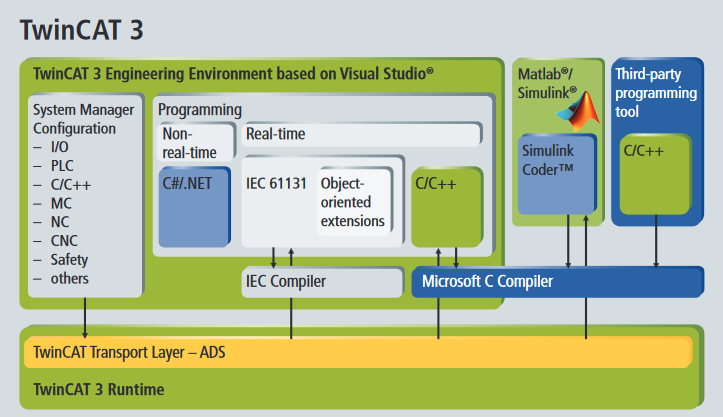
\includegraphics[width=0.90\textwidth]{Pictures/TwinCat3_Beckhoff.png}
\caption{TwinCAT 3 \citep{Beckhoff2016}}
\label{fig:TwinCAT}
\end{figure}


Die im vorherigen Abschnitt vorgestellte Statusmaschine soll mittels einer SPS-Programmierung umgesetzt werden. Zur informationstechnischen Umsetzung wurde die Automatisierungssoftware TwinCAT 3 der Fa. Beckhoff verwendet. TwinCAT ist die Abkürzung von \textit{The Windows Control and Automation Technology} und  ist in die Entwicklungssoftware \textbf{Visual Studio} der Fa.  von Microsoft integriert. Über das Visual Studios wird der Programmcode kompiliert, debugged, ausgeführt und überwacht. Sie ermöglicht es, den lokalen PC mit der SPS zu verbinden. 

TwinCAT 3 unterteilt sich hauptsächlich in zwei Unterpunkte: 

\begin{itemize}
\item	\textit{eXtended Automation Engineering} (XAE)
\item	\textit{eXtended Automation Runtime} (XAR).
\end{itemize}

Abbild \ref{fig:TwinCAT} zeigt den softwaretechnischen Aufbau von TwinCAT 3 sowie deren Schnittstellen und Unterstrukturen.

Das \textit{eXtended Automation Engineering} (XAE) ermöglicht durch ihre Orientierung an der IEC 61131-3 \footnote{IEC 61131-3:  Europäische Norm die sich mit den Grundlagen speicherprogrammierbarer Steuerungen bezüglich Programmiersprachen befasst.} die Verwendung von folgenden Sprachen :

\begin{itemize}
\item	Anweisungsliste (AWL)
\item	Kontaktplan (KOP)
\item 	Funktionsbaustein-Sprache (FBS)
\item	Ablaufsprache (AS)
\item	Strukturierter Text (ST).
\end{itemize}

Über die Norm-Programmiersprachen hinaus ist es möglich, echtzeitfähige, externe C++- Programme als auch nicht echtzeitfähige Programme mit VB.NET  als Programmiersprache in das Projekt einzubinden. Eine weitere Software-Schnittstelle erlaubt eine Verbindung zu  Toolboxen wie \textit{MATLAB} oder \textit{Simulink}. Des Weiteren eignet sich diese Schnittstelle zur Herstellung von einer Verbindung zu Datenbank-Software wie z. B.\textit{ MySQL} oder \textit{MariaDB}. Die erzeugten Objekte, auch Module genannt, können unabhängig von ihrer Programmiersprache, in der sie erzeugt wurden,  Daten austauschen und sich gegenseitig aufrufen. 

\textit{eXtended Automation Engineering} beinhaltet das Daten-Analyse-Programm \textit{Scope}. Wie auch TwinCAT selber ist \textit{Scope} in Microsofts Visual Studios eingebunden. Das \textit{Scope} unterteilt sich in \textit{Scope View} und \textit{Scope Server}. \textit{Scope View} erlaubt die Echtzeitdarstellung von Messdaten.  \textit{Scope Server} ist für die eigentliche Aufnahme der Daten verantwortlich.


\textit{eXtended Automation Runtime} (XAR) ist zuständig für die Kommunikation von allen angeschlossenen Geräten, Feldbussen und Busklemmen der SPS. Das (XAR) stellt einen Durchlauf des gesamten Programmcodes sowie das Empfangen und Senden einer Busklemme-Signals innerhalb eines Zyklus sicher. Auf einer SPS können mehrere Tasks laufen. Jedem Task wird eine Dauer und eine Priorität durch den Benutzer zugeteilt. Der Task mit der höchsten Priorität wird stets zuerst ausgeführt. Auf dem verwendeten CX-9020 können maximal 4 Tasks ausgeführt werden. Ein Task besteht aus einem oder mehreren Programmen, Funktionen und Funktionsbausteinen.  Die Grundlage jeglicher Kommunikation ist das \textit{Automation Device Specification} (ADS). Es stellt eine geräte- und feldbus-unabhängige Schnittstelle zwischen ADS-Teilnehmern dar. 
